\documentclass[scheme=plain,12pt]{ctexart}

\usepackage{graphicx}
\usepackage{amsthm}
\usepackage{amsmath}
\usepackage{amssymb}
\usepackage[hmargin=1.1in,vmargin=1in]{geometry}
\usepackage{indentfirst}
\usepackage[defaultmono,scale=0.85]{droidsansmono}
\usepackage{color}
\usepackage{minted}
\usepackage{multirow}
\usepackage[xetex,colorlinks=true]{hyperref}

\fontsize{14pt}{1.0}
\definecolor{codebg}{rgb}{0.95,0.95,0.95}

\newlength{\blanklength}
\setlength{\blanklength}{40ex}

\providecommand{\thetitle}{Project 03}
\providecommand{\theauthor}{Sparky\_14145}
\providecommand{\thestudentID}{71XXXXXX}
\providecommand{\theemail}{Sparky\_14145@outlook.com}
\providecommand{\theinstitution}{College of Software Engineering}

% \input{personal_info/info.tex}

\providecommand{\blankToFill}[1]{
    \parbox[t][3ex]{\blanklength}{
        \makebox[\blanklength]{#1}\\[0pt]
        \rule[2ex]{\blanklength}{0.1ex}
    }
}

\providecommand{\makecover}{\begin{titlepage}
    \noindent
    {Project Report} \\[2pt]
    {\large \bfseries Southeast University}

    \vspace*{70pt}
    \begin{center}
        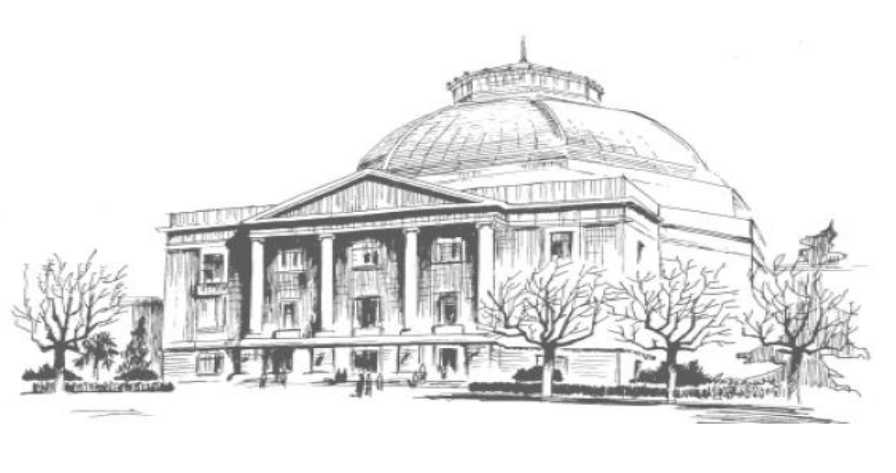
\includegraphics[width=0.9\textwidth]{pics/cover.png} \\[2pt]
        \textsc{\Huge Principles of Databases}\\[10pt]
        \begin{tabular}[c]{rc}
            Title       & \blankToFill{\thetitle} \\
            Date        & \blankToFill{\today} \\
            Author      & \blankToFill{\theauthor\footnotemark} \\
            Student ID  & \blankToFill{\thestudentID} \\
            Institution & \blankToFill{\theinstitution}
        \end{tabular}
        \rmfamily
    \end{center}
    \footnotetext{\theemail}
\end{titlepage}}

\begin{document}
    \makecover

    \tableofcontents
    \newpage

    \section{Background}

    Questionnaires are used much in our daily lives.

    This project will provide basic support to a simple questionnaire system, that allow users
    create, collect, manage and analyse questionnaires.

    \section{Functions}

    \begin{enumerate}
        \item User registration and account management;
        \item Questionnaire creation, cloning and modification;
        \item Customizing questions;
        \item Answer collection and analysis;
        \item Questionnaire multiple modification.
    \end{enumerate}

    \section{E-R Graph}

    \begin{figure}[hp]
        \centering
        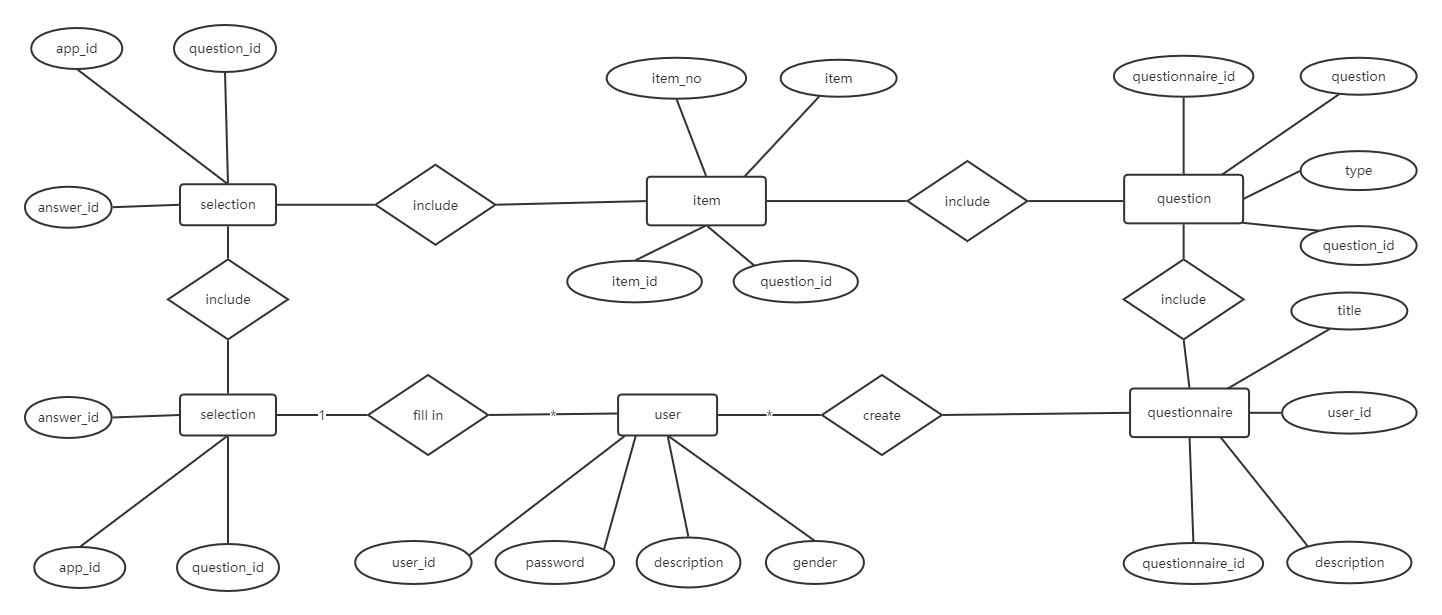
\includegraphics[width=0.9\textwidth]{pics/er-graph.png}
        \caption{E-R Graph of System}
        \label{fig:er-graph}
    \end{figure}

    \section{Schema}

    \begin{center}
        \begin{tabular}{|c|c|c|}
            \hline
            Table & Item & Explain \\ \hline
            \multirow{4}{*}{user} & user\_id & \textbf{Primary key}. The id of user. \\ \cline{2-3}
             & password & Password of the user. Used for authentication. \\ \cline{2-3}
             & description & User-defined self description. \\ \cline{2-3}
             & gender & Gender of the user. 0---secret, 1---male, 2---female. \\ \hline
            \multirow{3}{*}{questionnaire} & questionnaire\_id & \textbf{Primary key}. Id of questionnaire. \\ \cline{2-3}
             & title & The title of the questionnaire \\ \cline{2-3}
             & description & Description of the questionnaire \\ \hline
            \multirow{5}{*}{question} & question\_id & \textbf{Primary key}. Id of question. \\ \cline{2-3}
             & question & The question description. \\ \cline{2-3}
             & type & Type of the question. 0---None, 1---Single Choice, \\
             & & 2---Multi Choice, 3---Essay Question \\ \cline{2-3}
             & questionnaire\_id & The questionnaire the question belongs to. \\ \hline
            \multirow{2}{*}{answer} & answer\_id & Id of the answer. \\ \cline{2-3}
             & user\_id & Id of the author of the answer. \\ \hline
            \multirow{5}{*}{selection} & selection\_id & \textbf{Primary key}. \\ \cline{2-3}
             & answer\_id & The answer this selection belongs to. \\ \cline{2-3}
             & question\_id & The question of this selection. \\ \cline{2-3}
             & selection & Item number if the question is a choice question, \\
             & & the answer text otherwise. \\ \hline
            \multirow{4}{*}{item} & item\_id & \textbf{Primary key}. \\ \cline{2-3}
             & question\_id & The question this item belongs to. \\ \cline{2-3}
             & item\_no & Number of this item. \\ \cline{2-3}
             & item & The item description. \\ \hline
            \multirow{3}{*}{owner} & record\_id & \textbf{Primary key}. \\ \cline{2-3}
             & user\_id & The user that can manage the questionnaire. \\ \cline{2-3}
             & questionnaire\_id & The questionnaire that to be managed. \\ \hline
        \end{tabular}
    \end{center}

    \section{Function Implementations}

    Only several complex functions are shown.

    \subsection{Show the selection count of items of a choice question}

    \begin{center}
        \small
        \inputminted[bgcolor=codebg,autogobble,linenos=true,breaklines]{sql}{src/fun1.sql}

        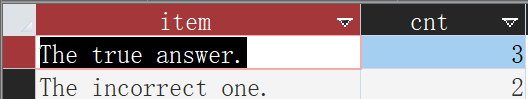
\includegraphics[width=0.4\textwidth]{pics/fun1.png}
    \end{center}
\end{document}